We build ranking models for Sports, Finance and News stream respectively, 
collecting two weeks of user action data for training and one week for test.  
Sports, Finance and News are big streams. Under them 
there are small streams such as NFL,NBA,MLB from Sports (see 
Fig.~\ref{hierarchy}). Data distribution are shown in Table.~\ref{data 
distribution}. The table shows the number of clicks and views for different 
properties in our training and test data. 



\begin{table}
\begin{center}
\caption{Click data distribution}
 \label{data distribution}
\begin{tabular}{|c|c|c|c|c|c|c|}\hline
 &  \multicolumn{3}{c|}{training} & \multicolumn{3}{c|}{test} \\ \hline
property     & click & view & total & click & view & total\\ \hline
Sports &  108K & 1.5M  & 1.6M & 12K & 178K & 191K \\ \hline
NFL &   20K & 328K  & 347K & 1.5K & 21K & 22K \\ \hline
NBA  &  7K & 66K & 72K & 649  & 8K & 9K \\ \hline
MLB & 7K & 9K & 95K & 971 &14K & 15K \\ \hline
Finance & 57K & 779K  & 836K & 5K &73K & 79K \\ \hline
News & 109K & 1.4M &1.5M  &14K &207K &221K \\ \hline
\end{tabular}

\end{center}

\end{table}


GBDT is our learning method of choice.  The comparisions between GBDT and 
linear regression under different feature size  are shown in 
Table~\ref{phase2sum}. We take as our baseline model linear regression with 
features from Phase 1 (equal to "flat gmp'' as in Table~\ref{tag:phase1exp}). 
Note experiments on Phase 1 and Phase2 used distinct training set and test 
set. Hence, the numbers shown on Table~\ref{phase2sum} and 
Table~\ref{tag:phase1exp} are not aligned. Two GBDT model results are shown 
here. One uses phase 1 features and the other uses a total of 14 Phase 2 
features as described in Section~\ref{sec:phase2}.  The same algorithm is 
applied to three distinct top-level properties: Sports, Finance and News. The 
linear baseline models gave the worst results. The GBDT with Phase 2 features 
yields the best results. We use Receiver Operating Chracteristics Area Under 
the Curve (AUC) as the principle metric.


\begin{table}
\caption{Comparision of Phase 2 ranking models}
\begin{tabular}{|c|c|c|c|}\hline
             & Sports & Finance & News \\ \hline
Base (linear phase1 feature) & 0.56 & 0.53 & 0.56 \\ \hline 
GBDT(Phase 1 feature)  & 0.59& 0.62& 0.58 \\ \hline
GBDT(Phase 2 feature) & 0.64 & 0.66 & 0.62 \\ \hline
\end{tabular}

\label{phase2sum}
\end{table}


Intuitively, one would assume that better results could be derived if each 
stream uses its own model. Actually, we found this to be true only for 
heterogeneous top level streams such as Sports, Finance and News, but no 
longer holds for 
relatively homogeneous steams such as NFL,NBA and MLB, all of which are 
sub-streams of Sports.  To show this, we trained a general model using all 
sports data, and a dedicated model for each sub-stream using only the data 
from each sub-stream. Accordingly, we test the models on test data from 
different streams. The results are shown in Table~\ref{tab:substream}. 

\begin{table}
\caption{Substream evaluations}
\begin{tabular}{|c|c|c|c|c|} \hline
    \diaghead{\theadfont training  test data}{training \\ data}{test  data}   & Sports & NFL & NBA & MLB \\ \hline
    Sports & 0.636 &0.629 &0.662 &0.705 \\ \hline
    NFL & - & 0.610 & - & - \\ \hline
    NBA & - & - & 0.645 & \\ \hline
   MLB & - & - & - & 0.676 \\ \hline
   with srcspaceid  & 0.642  & 0.635 &0.689 & 0.725 \\ \hline
\end{tabular}

\label{tab:substream}
\end{table}

We found that the model trained on all sports data performed better than 
dedicated models. 
We interpret this to mean that using all data can have rich feature 
distributions while feature distributions are biased for sub-streams. Simply 
increasing training data sizes can't satisfy rich feature distributions.  
Actually, the training data sizes we used for sub-stream models are 
sufficient 
to achieve maximal performance. As shown in Fig.~\ref{fig:curve}, it is a 
training curve which shows the trend of AUC change on the same test set as 
increasing training data size. The training data size is large enough to make 
the maximal results, which proves increaing more training data size does not 
help.  

\begin{figure}
\caption{Test data metrics as increasing sub-stream training data 
size}\label{fig:curve}
%\centering 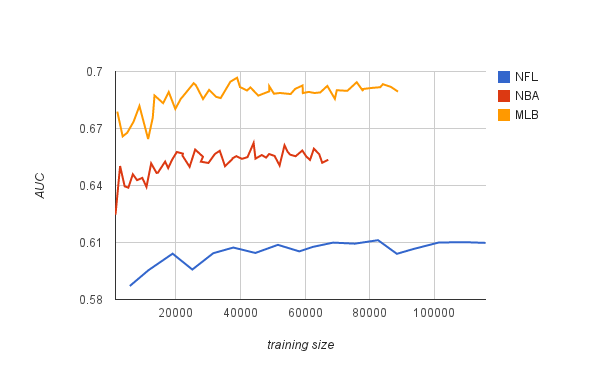
\psfig{file=training-curve.png,width=3.3in,}
\centering
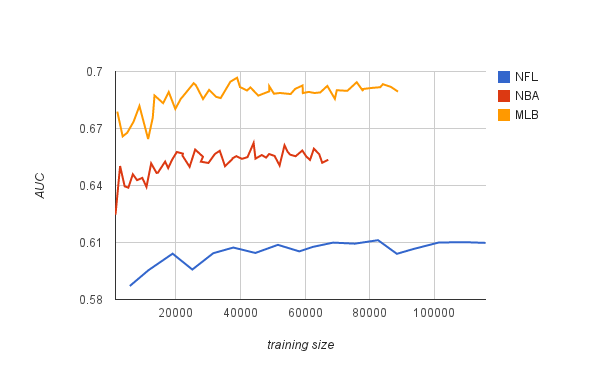
\includegraphics[width=3.5in]{training-curve.png}

\end{figure}

We found that using stream-id as feature can improve substream ranking. This 
is a categorical feature for multiple stream ranking. Each decision tree in 
the GBDT ensemble can be split at node with logic such as stream-id $\in 
\{NFL,NBA\}$.  The model with these features is trained on all sports data.  
The results are even better than using all sports data. They are shown on the 
last line of  Table~\ref{tab:substream}. Ranking metrics are improved for all 
sub-streams with this additional feature.
 




  
 In addition to personalized relevance, ranking should also promote fresh 
 contents.  Indeed, if recency is not specifically treated,  many old articles 
 would be placed towards the top of the streams because old articles can 
 accumulate 
 higher popularity scores. On the other hand, recency can't be over-promoted.  
 Ranking solely by document age is a very bad idea because this will show many 
 low quality and irrelevant articles to users. Therefore, a balance between 
 relevance and recency needs to be considered.  Usually, there are two methods 
 in handling recency. First, as used in Phase 1, recency can be boosted by 
 applying an exponential age decay factor. Old age documents are punished.  
 Related works can be found in 
 \cite{Li:2003:TLM:956863.956951,Metzler:2009:ISR:1571941.1572085}. A second 
 option is to use document age as a feature. Recency feature is integrated 
 with other features. The relative importance of recency and relevance feature 
 is 
 completely determined by the training data and the algorithm. 
 
 We tested both methods, with results shown in table~\ref{recency}. Here we 
 take as 
 the baseline model the best ranking model from the previous expriments, 
 namely, GBDT with 14 phase-2 features.

\begin{table} 
\caption{ Recency evaluation }\label{recency}
\begin{tabular}{|p{50mm}|c|c|}\hline
     & AUC & age@top1 \\ \hline
Sports Base (Phase2 gbdt) &  0.64 & 10.3  \\ \hline
Sports (expontial age decay) & 0.58 & 7.5 \\ \hline
Sports (age as feature) & 0.66  & 8.3 \\ \hline \hline
%% Sports (age as feature) + expontial age decay & 0.62 & 6.5 \\ \hline  \hline
Finance Base & 0.66 & 6.6 \\ \hline
Finance (expontial age decay) & 0.60 & 4.6 \\ \hline
Finance (age as feature)  & 0.68 & 6.4 \\ \hline
%%Finance (age as feature) + expontial age decay & 0.64 & 4.2 \\ \hline
\end{tabular}

\end{table}

"age@top1" is the average document age (hour) of the first articles in the 
stream over all sessions. A session is the period from when a user comes to 
the site to when she leaves, or 30 minutes, whichever is shorter. 
For example, the average document age under the Sports baseline model is 10.3 
hours. The model "expontial age decay" discounts the baseline ranking score 
exponentially by document age, similar to the exponential multiplier $e^{\beta 
\Delta T}$ as in \eqref{practical SRQ}. The model "age as feature" used 
age simply as a feature in GBDT. 
%%The final one "age as feature + expontial age decay" applied expontail age decay over the results from "age as feature".  This is an effort to boost recency
We found that using document age as a feature achieves better results than 
using expontial age decay: both AUC (relevance metric) and age@top1 are 
improved while expontial age decay results in a big relevance drop in terms of 
AUC.
The results are consistent for both Sports and Finance streams. 


We also did online user experience test (bucket test) to evaluate GBDT models 
(Table~\ref{bucket test}). We were able to do bucket test for Sports and 
Finance at the time. The models were compared to a linear ranking model (as 
Phase 1). Both CTR and Dwelltime improved by more than double digits. 

\begin{table}
\caption{bucket test}
\begin{tabular}{|c|c|c|}\hline
             & CTR & Dwell time  \\ \hline
Base (Linear) &  - & -   \\ \hline 
Sports,GBDT(phase 1 feature)    & +6\% & +6\% \\ \hline
Sports,GBDT(Phase 2 feature) & +25\% & +21\% \\ \hline
Finance,GBDT(phase 1 feature)  & +3\% & +3\% \\  \hline
Finance,GBDT(Phase 2 feature) & +20\% & +18\%  \\  \hline
\end{tabular}

\label{bucket test}
\end{table}






